\documentclass[11pt]{article}
\usepackage{graphicx}
\usepackage{subfigure}
\usepackage{hyperref}
\usepackage{listings}
\usepackage{float}
\usepackage[a4paper, total={6in, 8in}]{geometry}

% Title Page
\title{INF560 $\cdot$ Image Filtering}
\author{Delacourt Remi $\cdot$ Amponsem Kwabena}


\begin{document}
\maketitle
\begin{center}
    \href{https://github.com/Flechman/X-INF560-Project}{GitHub repository to the project source code}
\end{center}
\newpage
\tableofcontents
\newpage

\section{Introduction}
\subsection{Report setting}

In this project, data parallel computation techniques were used to improve the performance of an image filtering program. In the sequential version, a GIF image is accepted as input and then an output, after filtering, is generated.
\begin{figure}[h]
	\centering
	\subfigure[]{
\includegraphics[scale=0.1]{original.png}}
	\subfigure[]{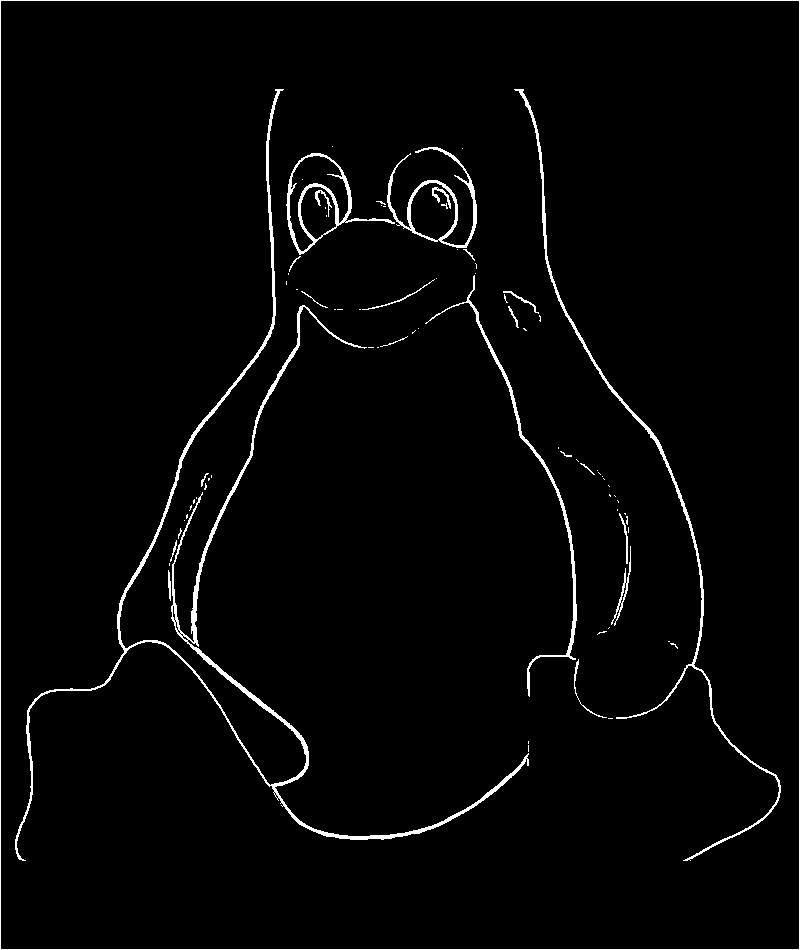
\includegraphics[scale=0.1]{processed.png}}
	\caption{(a) Original GIF image (b) Processed GIF image}
	\label{fig:introduction}
\end{figure}

To parallelize the sequential version, several parallelization models were studied and after vigorous investigation, the models were incorporated. \\
In the report we make a difference between animated Gif and image : an animated gif is a full gif input, whereas an image is part of the animated gif. Each animated gif contains multiple images. \\
\\
The report is structured as follows:
\begin{itemize}
	\item An in-depth explanation of the implementation of the parallel algorithms of the program (using MPI, OpenMP, and CUDA).
	\item Performance evaluation by comparing the parallel version against the sequential version.
	\item Some improvements that could be made on top of our implementation, for even better performance.
\end{itemize}

\subsection{Running the program}
\begin{center}
    \href{https://github.com/Flechman/X-INF560-Project}{GitHub repository to the project source code}
\end{center}

\begin{itemize}
    \item Navigate to the Project's root directory
    \item Navigate to the \textbf{Parallelized} folder
    \item You will find a shell script named \textbf{run\_test.sh}.
    \item In order to run the program, these arguments would have to be passed along: 
    \begin{enumerate}
        \item \textbf{-n} $\{$Number of MPI Processes$\}$
        \item (\textbf{-N} $|$ Optional) $\{$Number of nodes$\}$
        \item (\textbf{-t} $|$ Optional) $\{$values: $\langle$\textit{"mpi"},\textit{"mpi\_omp"}$\rangle$ $\}$
        \item (\textbf{-o} $|$ Conditional: used alongside \textbf{-t} \textit{mpi\_omp}) $\{$Number of OpenMP threads$\}$.
    \end{enumerate}
    \textbf{NB:} All commands are passed without curly brackets '{}'.
\end{itemize}

\section{Implementation}

In this section, we give an in-depth explanation of the parallel algorithms employed in the project.
We started adding MPI, then we added openMP, and finally we tried to add CUDA. Since the results with CUDA weren't satisfying compared to only MPI + openMP, we've decided not to keep it, and we will give an explanation and show why our CUDA incorporation wasn't efficient.

\subsection{MPI}

\subsubsection{Parallelism approach & choices}
To incorporate MPI into our program, we needed an algorithm to split the animated gif into sub-images and have a structure that would be scalable for the filtering part of the program.
Since we work in a distributed memory setting, after splitting we had to distribute the resulting sub-images.

We chose to keep the animated gif structure to represent the sub-images, to have a sort of composite design pattern, and so every process would work on an animated gif structure.

The algorithm we went for to split the image is the following : \\
Process 0 (the master process) retrieves the full image in a sequential manner just like the sequential version of the program. Then a distribute function is called, which will be in charge to split the image and distribute it among the other processes. The splitting is done on the height of each image, that way each process works on $1/n$ portion of each image in the animated gif ($n$ is the number of processes). \\
We chose to put MPI on the height of images instead of width because in the blur filter function, most of the computation is done on the top 10\% and on the bottom 10\% of each image. By dividing images on the height we reduce the potential communications between processes because potential communication will only occur in 20\% of each image.
Figure \ref{fig:overview} shows well how the splitting is done. \\
\\
\begin{figure}[H]
	\centering
	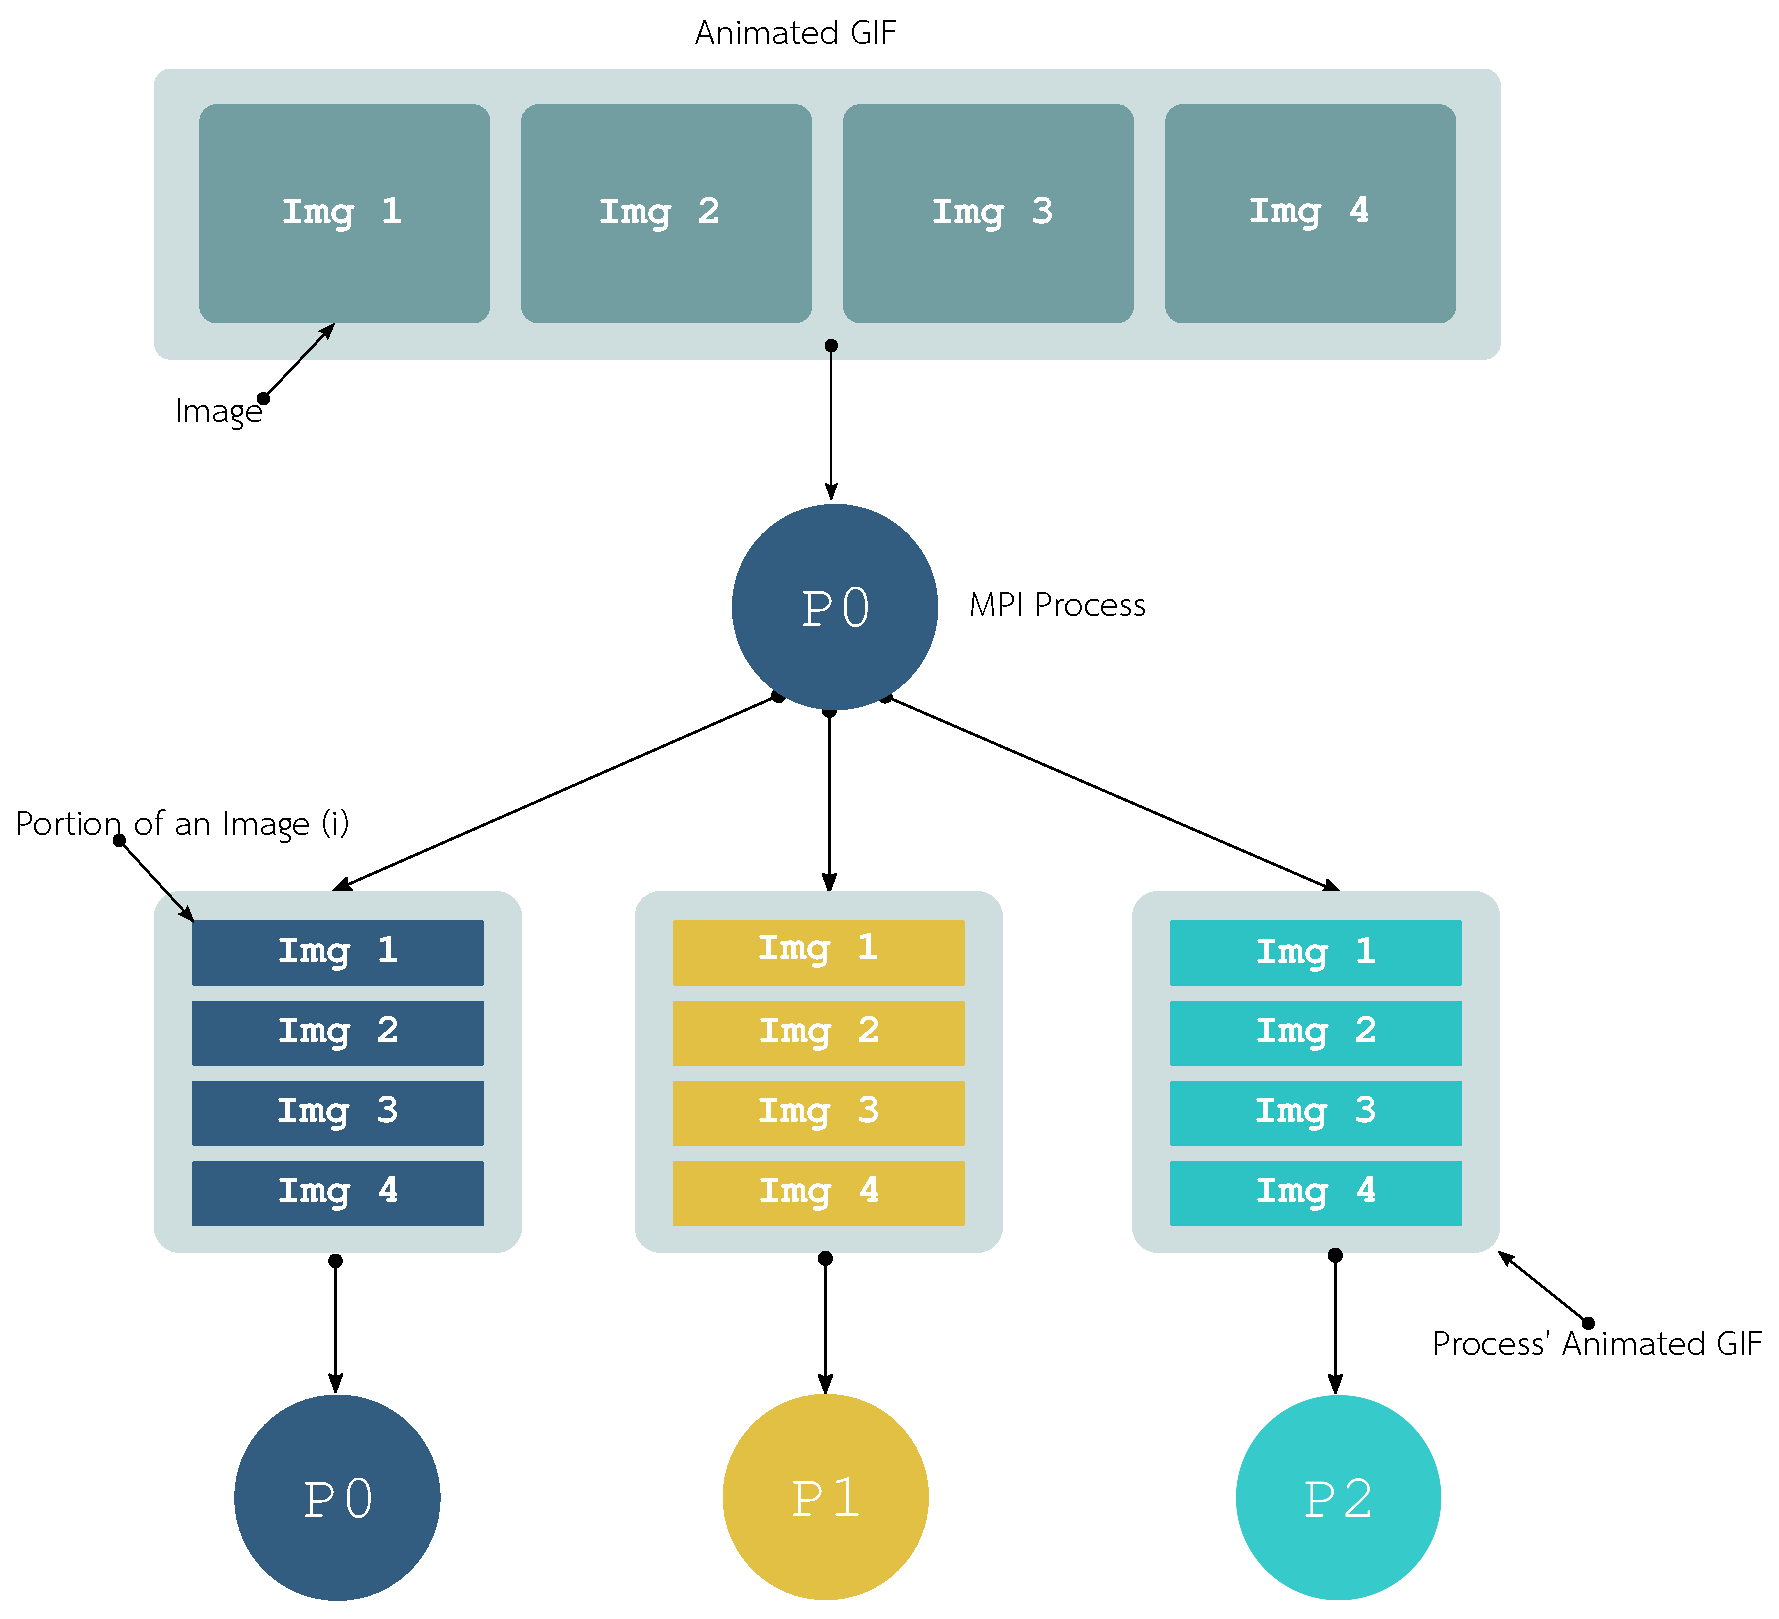
\includegraphics[scale=0.45]{INF560-Image-Filtering-EPS.eps}
	\label{fig:overview}
	\caption{High-level abstraction of the parallel algorithm.}
\end{figure}
In our model, each image in the animated GIF is split according to the number of processes. This means that considering Figure \ref{fig:overview}, since there three (3) processes, each \textit{Img} would be divided into three portions along the height of the image, color coded as \textit{dark blue}, \textit{yellow}, and \textit{light blue}.
In that sense, each process would have a new animated gif consisting of smaller chunks of all the individual images in the animated gif. \\\\
It is important to note that process 0 will sequentially distribute the image, meaning that some processes will do nothing for some time and just wait for process 0 to send their image part. This cannot be avoided since a process needs its part of the image to be  able to work. But one could argue that it is better than letting every process retrieve at once their part of the image directly from the file system, because doing this would lead to too much I/O overhead. \\
\\
This way of splitting is particularly interesting for the blur filter function, which is the main actor in the overall runtime of the program. This is because in the blur filter we work on one image of the animated gif at a time, and having to deal with a while loop per image makes the blur function implementation difficult to change. So if each process works on one image at a time and on the same image, then communication between processes becomes much  easier.
\\
\begin{figure}[H]
	\centering
	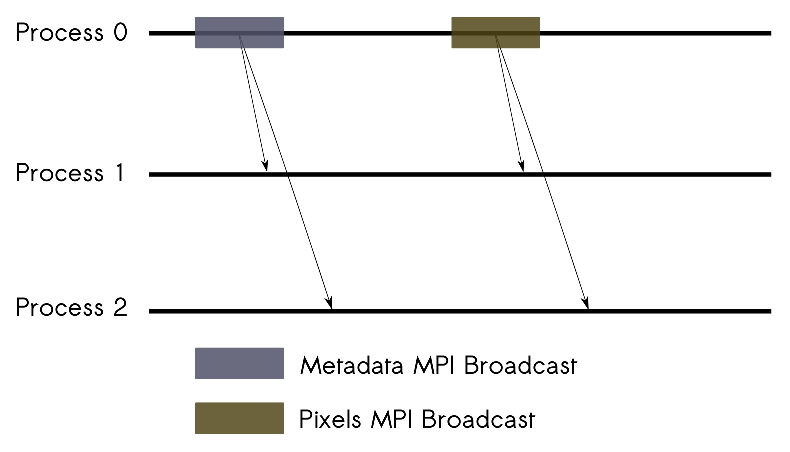
\includegraphics[scale=0.6]{MPI_Bcast.eps}
	\caption{The master process sending broadcasting data to other processes.}
\end{figure}
\subsubsection{Experimental evaluations}
\begin{figure}[h]
	\centering
	\subfigure[]{\includegraphics[scale=0.55]{THREADS_PROCESSES_OUTPUT_FILE.eps}}
	\subfigure[]{\includegraphics[scale=0.55]{THREADS_PROCESSES_OUTPUT_FILE2.eps}}
	\caption{(a) 1 to 12 processes (b) 13 to 20 processes}
	\label{fig:MPIeval}
\end{figure} \\
Figure \ref{fig:MPIeval} shows the runtime evolution of the filter part of the program on the biggest image of our dataset, the campus map of the university of Hohenheim, as the number of processes increases. We can see that as we increase the number of processes, the runtime of the filter decreases, which confirms the efficiency of our MPI implementation.\\
\begin{figure}[h]
	\centering
	\includegraphics[scale=1.0]{RESULTS_MULTI_1,1,20_procs_1,1,1_threads.eps}
	\caption{Graph showing the runtimes on the provided dataset of images. Colors represent a run with a certain number of processes.}
	\label{fig:MPIevalGraph}
\end{figure}
Figure \ref{fig:MPIevalGraph} shows us the general trend of the runtimes. We see that MPI still has its limitations in improving the performance, as most of the runtimes are around the same values.

\newpage

\subsection{OpenMP}
\subsubsection{Parallelism approach & choices}
To add to our distributed memory setting with MPI, we've added parallelism using the shared memory model with OpenMP. \\
Since we've already used MPI to parallelize on the  height of each image, we intuitively parallelized with OpenMP on the width.

Looking at the runtime of the different parts and steps of the program, the blur filter seems to be the bottleneck by far (on average 5 to 10 times longer than the Sobel filter). Se we decided to focus on it and use OpenMP exclusively on it. After all, using OpenMP in other parts of the program won't make a difference on the overall runtime before utilizing it in the blur filter. 

A first approach we had was to add parallel regions at every for loops we encountered in the blur filter, and then dividing the loop and distributing it among the threads. This resulted in bad parallelism for two main reasons : it is expensive to create a parallel region (fork + join); everything is done in a while loop, so creating and ending all these parallel regions at each while loop iterations is even more expensive and time-consuming. Overall the runtime was worse than the one with  just MPI. 

We  then thought of another solution learning from the previous issues that would create a single parallel region that would contain the while loop. Unfortunately, this required to synchronize a lot the threads throughout the code in the while loop because of dependencies, and finally the performance wasn't really improved. 

An intermediate solution was then to refactor the code as follows : in the while loop, all of the MPI communication is done at the beginning, and all the computation loops (the most time-consuming parts) are grouped in a single code block. That way, at every while loop iteration, a single OpenMP parallel region is created, and the loops are parallelized. \\
This final version was the best solution we found for parallelizing the blur filter with OpenMP.

Furthermore, since in each for loops where we compute the new values of the pixels we write on disjoint parts of memory, we don't need to make some synchronization between the threads at this level, so we don't get any additional cost. \\
Between the for loops, it is still required to synchronize the threads using implicit barriers because some for loops are dependant on previous ones. 

Static OMP loop scheduling was employed because the number of iterations of each \textit{for} loop is similar or close to similar (because we iterate on the width), and the work of each \textit{for} loop is uniformly distributed among each iteration. Using a dynamic schedule wouldn't lead to better performance because it adds some unnecessary complexity. \\

\subsubsection{Experimental evaluations}
\begin{figure}[H]
	\centering
	\includegraphics[scale=0.9]{THREADS_PROCESSES_OUTPUT_FILE3.eps}
	\caption{Runtime evolution from 1process:1thread to 10processes:8threads}
	\label{fig:OMPeval}
\end{figure}
Figure \ref{fig:OMPeval} shows the runtime evolution of the filter part of the program on the biggest image of our dataset, the campus map of the university of Hohenheim, as the number of processes and the number of threads increases. We can see that starting at around 6 processes and 8 threads the runtime increases back. This shows balance between the cost of distributing computation, and the cost of computing without further distribution.\\
\begin{figure}[H]
	\centering
	\includegraphics[scale=1.0]{RESULTS_MULTI_1,1,10_procs_1,1,8_threads.eps}
	\caption{Graph showing the runtimes on the provided dataset of images. Colors represent a run with a certain number of processes and threads.}
	\label{fig:OMPevalGraph}
\end{figure}
Just as in MPI we obtain runtimes that stay arount the same value, so a balance can be found between the number of resources used and the actual runtime increase we get from these resources. \\

\subsection{CUDA}
To incorporate CUDA in the program, we again looked at the distribution of the runtime among the different functions, and we concentrated ourselves on the blur filter. \\
We removed the OpenMP part in the blur and used CUDA for the exact same block of code. The reason for it is that we tried not to mix MPI communications with CUDA devices. 

The runtime with CUDA and MPI was bad compared to MPI+OpenMP, we obtained a performance decrease. There may be many reasons for that : every process will communicate and send its data to its respective CUDA device and it is very expensive to send the data accross the network to a CUDA device; The CUDA devices are summoned at each while loop and there is a while loop for each image of the animated gif. 

Furthermore, as the number of MPI processes increases, the runtime increases. Here are some runtime results : \\
\begin{figure}[H]
	\centering
	\includegraphics[scale=1.0]{RESULTS_2,2_MPI_OMP_CUDA_Perf_Analysis_regular.eps}
	\caption{Graph showing the runtimes on the provided dataset of images. 2 MPI processes used, with 2 CUDA devices (1 for each process)}
	\label{fig:CUDAeval}
\end{figure}
\\
Finally, we chose not to keep the CUDA implementation and we kept the previous version of the file. One could argue that using CUDA for such a project is not the best to explore the full capabilities of GPU programming, but there is definitely room to improve and get a performance increase here. \\
We have provided the source code of the program using CUDA (mainparaV2.cu), although it does not play a role in our actual parallel run. \\
\newpage
\section{Room for improvement}
One drawback of our code is that at a certain number of processes N available for the program (this number is dependent on the size S of each image of the animated gif and on the blur radius R), some processes will not work: when $S < R*N$. This is because the logic of the blur filter does not support that. Having this inequality above would mean too many communication between processes, and we reach a point where the time for communication added to the time for small computation is greater than just the time for bigger computation. \\
There is a solution for this issue which makes the code even more complex, but for deadline reasons we didn’t implement it. Here is a potential solution : if N is n times greater than the number of processes used for the program, split the set of images in the animated gif into n+1 subsets of images. For each subset, use $N/n$ processes to work on this subset. A similar reasoning can be applied to less perfect cases. \\
\\


\section{Conclusion}

In this project, several approaches were studied to parallelize an important algorithm in visual computing, a field which requires computations to go fast. We've finally managed to increase the performance of the program and half the runtime on our dataset of images with few parallel resources. \\
However, depending on the topology of the images we're dealing with, the runtime may still vary. \\ 
\end{document}          
